\section{Visualization and Visual Analytics}

\todo{reconsider the first two subsections to move some parts to Introduction}
\subsection{Visualization}
Defines vis~\cite{Munzner2014}. difference between scivis and infovis. Classic example: Minard's map of Napoleon's march.

How does vis support analysis?~\cite{Card1999} Classic example Anscombe's quartet

The value of vis (Wijk, Fekete)

vis reference model~\cite{Card1999}


\subsection{Visual Analytics}
Define v/a~\cite{Thomas2005, Keim2010}

Describe visual analytics process model (Figure~\ref{fig:visual-analytics-process})

\begin{figure}[!htb]
	\centering
	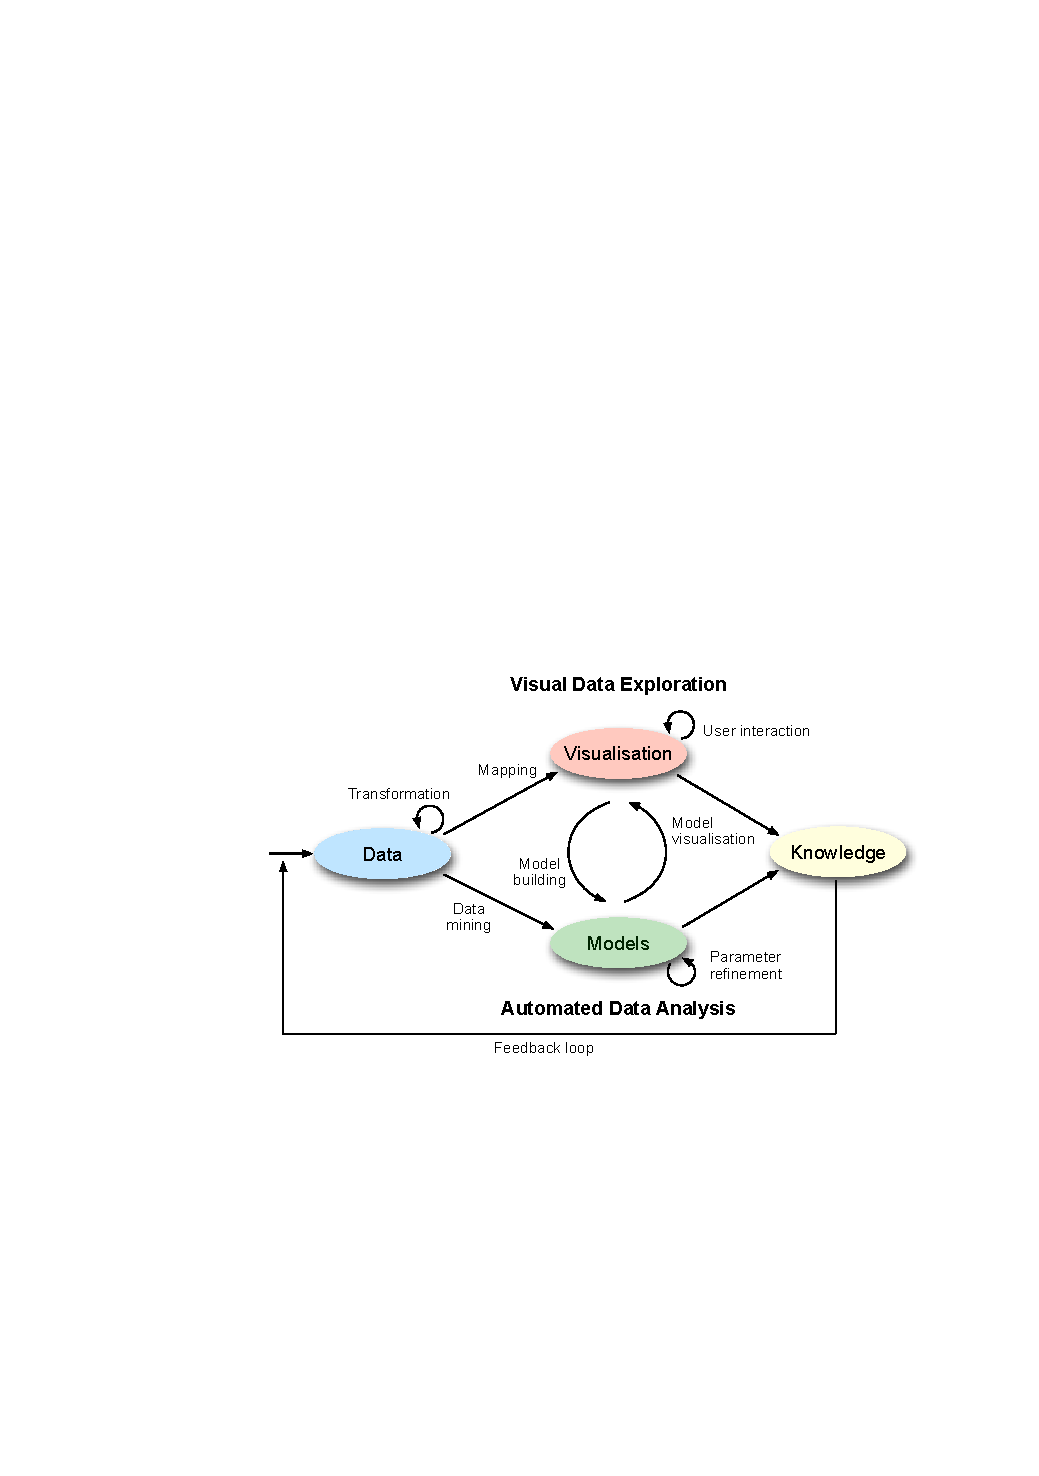
\includegraphics[width=\columnwidth]{visual-analytics-process}
	\caption{The visual analytics process model. \emph{Source:~\cite{Keim2010}}.}
	\label{fig:visual-analytics-process}
\end{figure}

%some components of visual analytics (from William's slides) (they're similar to the new definition of visual analytics in Mastering the Information Age
%"Visual analytics combines automated analysis with interactive visualizations for an effective understanding, reasoning and decision making on the basis of very large and complex
%datasets.")
%\begin{itemize}
%	\item data analysis/data mining
%	\item interactive dynamics (Heer and Shneiderman) 
%	\item assembly of evidence, argumentation (toulmin, wigmore)
%\end{itemize}

Next, we discuss three essential aspects of visualization research that also contribute to our proposed solutions described in upcoming chapters: information design principles, interaction techniques, and methods to evaluate visualizations.

\subsection{Information Design Principles}
Structure of this section:

\begin{enumerate}
	\item Discuss visual channels that are used to represent individual data items, and the channel rankings	encoding channel ranking (Section 5.4.2 Munzner book)
	\item Discuss a special channel -- color -- that is commonly used in both numerical and categorical data. This channel is heavily used in our designs described in upcoming chapters.
	\item Discuss Gestalt principles that are used to represent groups of data items
	\item Putting things together, Tufte's design principles for a well-design graphic
	\item In a broader context, GUI design principles:  Schneiderman~\cite{Shneiderman2016} (eight golden rules), Norman (six design principles) ~\cite{Norman2002} and	Nielsen (ten usability heuristics)~\cite{Nielsen1994} -- create a table with rows showing similar principles
\end{enumerate}



%http://www.csun.edu/science/courses/671/bibliography/preece.html
%https://faculty.washington.edu/jtenenbg/courses/360/f04/sessions/schneidermanGoldenRules.html
%https://www.interaction-design.org/literature/article/shneiderman-s-eight-golden-rules-will-help-you-design-better-interfaces

%\subsubsection{Gestalt Principles}
%\label{sub:lr-gestalt}
%
%\subsubsection{Color}
%
%\subsubsection {Color Spaces}
%RGB and HSL
%
%\subsubsection {Colormaps}
%
%categorical
%sequential
%diverging

%Working memory becomes an important factor as it organise and process information
%when learning occurs (Global, 2000). Here information is sorted and organised into
%relevant schema. Schemas can be referred to as models or hypothetical structures
%that organises once knowledge of the world.
%
%perception for design, Colin Ware book
%

\subsection{Interaction Techniques}
What is interaction?~\cite{Pike2009a} Why is it useful?~\cite{Munzner2014}. 

Give examples from standard graphical user interfaces: highlight, zoom, scroll to vis-specific ones: brushing/linking, focus+context. [Use pictures for the vis-specific].

Some taxonomies: [make a table to show similar techniques in the same row]
\begin{itemize}
	\item Dix and Ellis~\cite{Dix1998}: Highlighting and focus, accessing extra
	information -- drill down and hyperlinks, overview
	and context -- zooming and fish-eye views, same representation / changing
	parameters, same data / changing representation,
	linking representation – temporal fusion
	\item Keim~\cite{Keim2002}: Dynamic projections, interactive filtering,
	interactive zooming, interactive distortion,
	interactive linking and brushing
	\item Wilkinson~\cite{Wilkinson2005}: Filtering, navigating (zooming/panning/lens),
	manipulating (node dragging/categorical
	reordering), brushing and linking, animating, rotating, transforming
\end{itemize}

Interaction is executed to achieve some goal, thus can also be classified based on its intent. Give an example that several techniques are used to serve a single purpose. This kind of classification helps visualization designers select suitable interaction techniques to serve for the capabilities they want to offer to the users.

%For example, unfolding sub-categories in an interactive pie
%chart [15], drill-down in a treemap [36], and semantic zooming [32]
%all may appear very different, but we argue that they serve the same
%purpose, getting more details.

\begin{itemize}
	\item Yi et al.~\cite{Yi2007}: 1) Select, 2) Explore, 3) Reconfigure, 4) Encode, 5) Abstract/Elaborate, 6) Filter, and 7)
Connect
	\item Heer and Shneiderman~\cite{Heer2012}:  Visualize. Filter. Sort. Derive. Select. Navigate. Coordinate. Organize. Record. Annotate. Share. Guide.
	\item Brehmer and Munzner~\cite{Brehmer2013}: encode, select, navigate, arrange, change, filter, aggregate, annotate, import, derive, record
\end{itemize}


%At one level, interaction typically refers to the set of controls
%provided to the user to manipulate an interface and the relationship
%between the user and that interface. At a more abstract level, there is the
%interaction between the user and the problem space. This higher-level interaction
%is a cognitive act that is enabled by computational tools, but it does
%not take place exclusively within them (nor, for that m
%
%
%Interactivity is crucial for building vis tools that handle complexity.
%When datasets are large enough, the limitations of both people
%and displays preclude just showing everything at once; interaction
%where user actions cause the view to change is the way forward.
%Moreover, a single static view can show only one aspect of
%a dataset. For some combinations of simple datasets and tasks,
%the user may only need to see a single visual encoding. In contrast,
%an interactively changing display supports many possible
%queries.
%In all of these cases, interaction is crucial. For example, an interactive
%vis tool can support investigation at multiple levels of detail,
%ranging from a very high-level overview down through multiple
%levels of summarization to a fully detailed view of a small part of it.
%It can also present different ways of representing and summarizing
%the data in a way that supports understanding the connections
%between these alternatives.

Discuss approaches that can improve many different interaction techniques: direct manipulation~\cite{Shneiderman1982, Kwon2011}, fluid interaction~\cite{Elmqvist2011}

Discuss cognitive utilities associated with interaction~\cite{Sedig2013} -- many techniques can facilitate sensemaking, reasoning, learning, etc.

Putting all together, combination of interaction techniques to explore data: Shneiderman's visual information seeking mantra: Overview first, zoom and filter, then details-on-demand~\cite{Shneiderman1996}. And an alternative approach suitable for large datasets: Search, Show Context, Expand on Demand ~\cite{VanHam2009}

\subsection{Evaluation of Visualizations}
Structure:
\begin{enumerate}
	\item what is evaluation and why is it important? (Munzner book)
%	\item different kinds of evaluation, taxonomies based on techniques~\cite{Carpendale2008}, design stages~\cite{Munzner2009}, scenarios~\cite{Lam2012}
	\item discuss the nested model of validation~\cite{Munzner2009} -- evaluation happens at different stages of the design process
	\item discuss the seven scenarios of evaluation ~\cite{Lam2012}
	\item discuss the 'user performance' scenario, which is used in TimeSets [refer to quantitative methods]
	\item discuss the 'visual data analysis and reasoning' scenario, or evaluating sensemaking, which is used in SL, SP, SM -- refer to the sensemaking measurement paper ~\cite{Wilson2013}[refer to qualitative methods]
\end{enumerate}


any particular kind you want to focus 
